% Insertar este fragmento en el informe principal.
% Las imágenes deben copiarse a la misma carpeta que el archivo .tex de Overleaf.

% Sección 4.3: Resultados del tablero de la consigna
\begin{figure}[htbp]
    \centering
    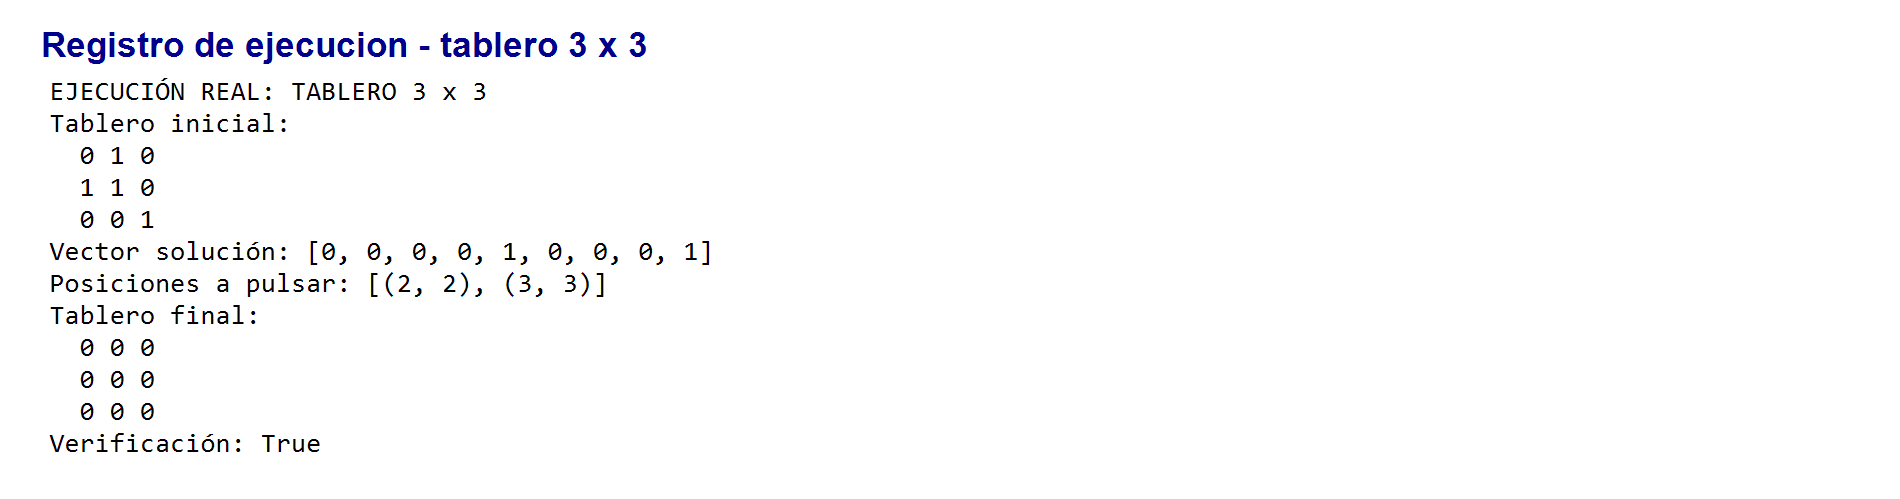
\includegraphics[width=0.92\textwidth]{evidencia/ejecucion_3x3.png}
    \caption{Ejecución del algoritmo para el tablero $3\times3$ de la consigna. Se observa el vector solución, las posiciones $(2,2)$ y $(3,3)$, el tablero final apagado y la verificación positiva.}
    \label{fig:ejecucion-3x3}
\end{figure}

% Sección 4.6: Pruebas automatizadas
\begin{figure}[htbp]
    \centering
    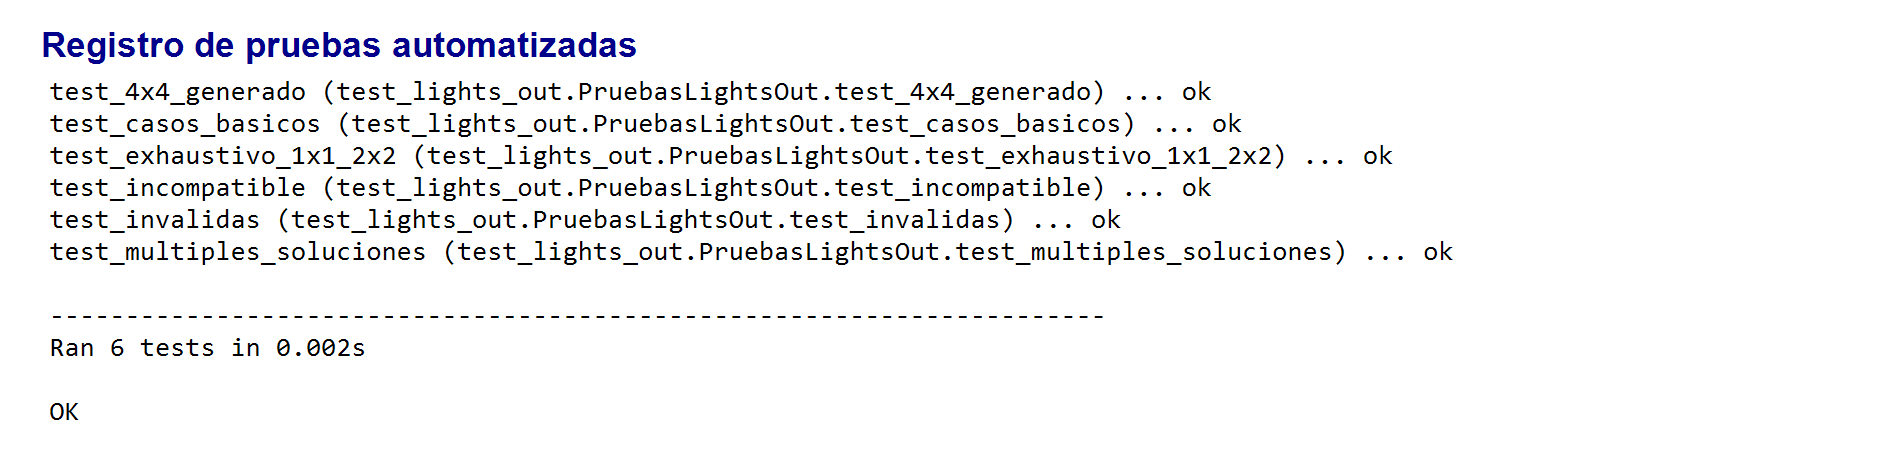
\includegraphics[width=0.92\textwidth]{evidencia/pruebas_automatizadas.png}
    \caption{Registro de la ejecución de las pruebas automatizadas del proyecto. Todas las pruebas finalizan correctamente.}
    \label{fig:pruebas-automatizadas}
\end{figure}
